\chapter{Object Detection}
L'Object Detection è un \textit{task} legato al mondo della \textit{computer vision}
che consiste nel rilevare e classificare istanze di oggetti in immagini o video.

Negli ultimi anni, grazie soprattutto all'avvento delle \ac{gpu}, c'è stato un 
incremento notevole del potere computazionale. Questo ha portato a sviluppare tecniche 
sempre più raffinate allo scopo di raggiungere prestazioni sempre migliori. 

Sempre grazie allo sviluppo di hardware sempre più potente l'interesse sta sempre 
più virando verso il mondo del \textit{Deep Learning}. 
In questo capitolo cercheremo di classificare le varie metodologie con cui si 
porta a compimento la \textit{Object Detection}. 
La letteratura sui detector è molto disomogenea e variegata, prenderemo quindi come riferimento i lavori di 
\textit{Licheng Jiao, Fan Zhang, Fang Liu, Shuyuan Yang, Lingling Li, Zhixi Feng and Rong Qu} 
\cite{DBLP:journals/corr/abs-1907-09408} e 
\textit{Zhengxia Zou, Zhenwei Shi, Yuhong Guo and Jieping Ye} \cite{DBLP:journals/corr/abs-1905-05055}.


\section{Storia della object detection}
\label{sec:history_obj}
Una prima, ma importante distinzione va fatta tra il periodo pre e post \textit{deep learning}. Il primo periodo va dagli inizi degli anni $2000$ fino al $2014$. Il secondo periodo, dove hanno preso il sopravvento tecniche basate sul \textit{deep learning}, va dal $2014$ fino ai nostri giorni. Quest'ultime tecniche possono essere a loro volta divise in altre due categorie, \textit{One Stage Detector} e \textit{Two Stage Detector} (sarà il caso di tradurre in italiano?) il cui sviluppo procede in maniera parallela. In Figura \ref{fig:history_object_detection} è presente uno schema riassuntivo con tutte le pietre miliari raggiunte durante lo sviluppo di tecniche per il rilevamento di oggetti.
\begin{figure}
    \centering
    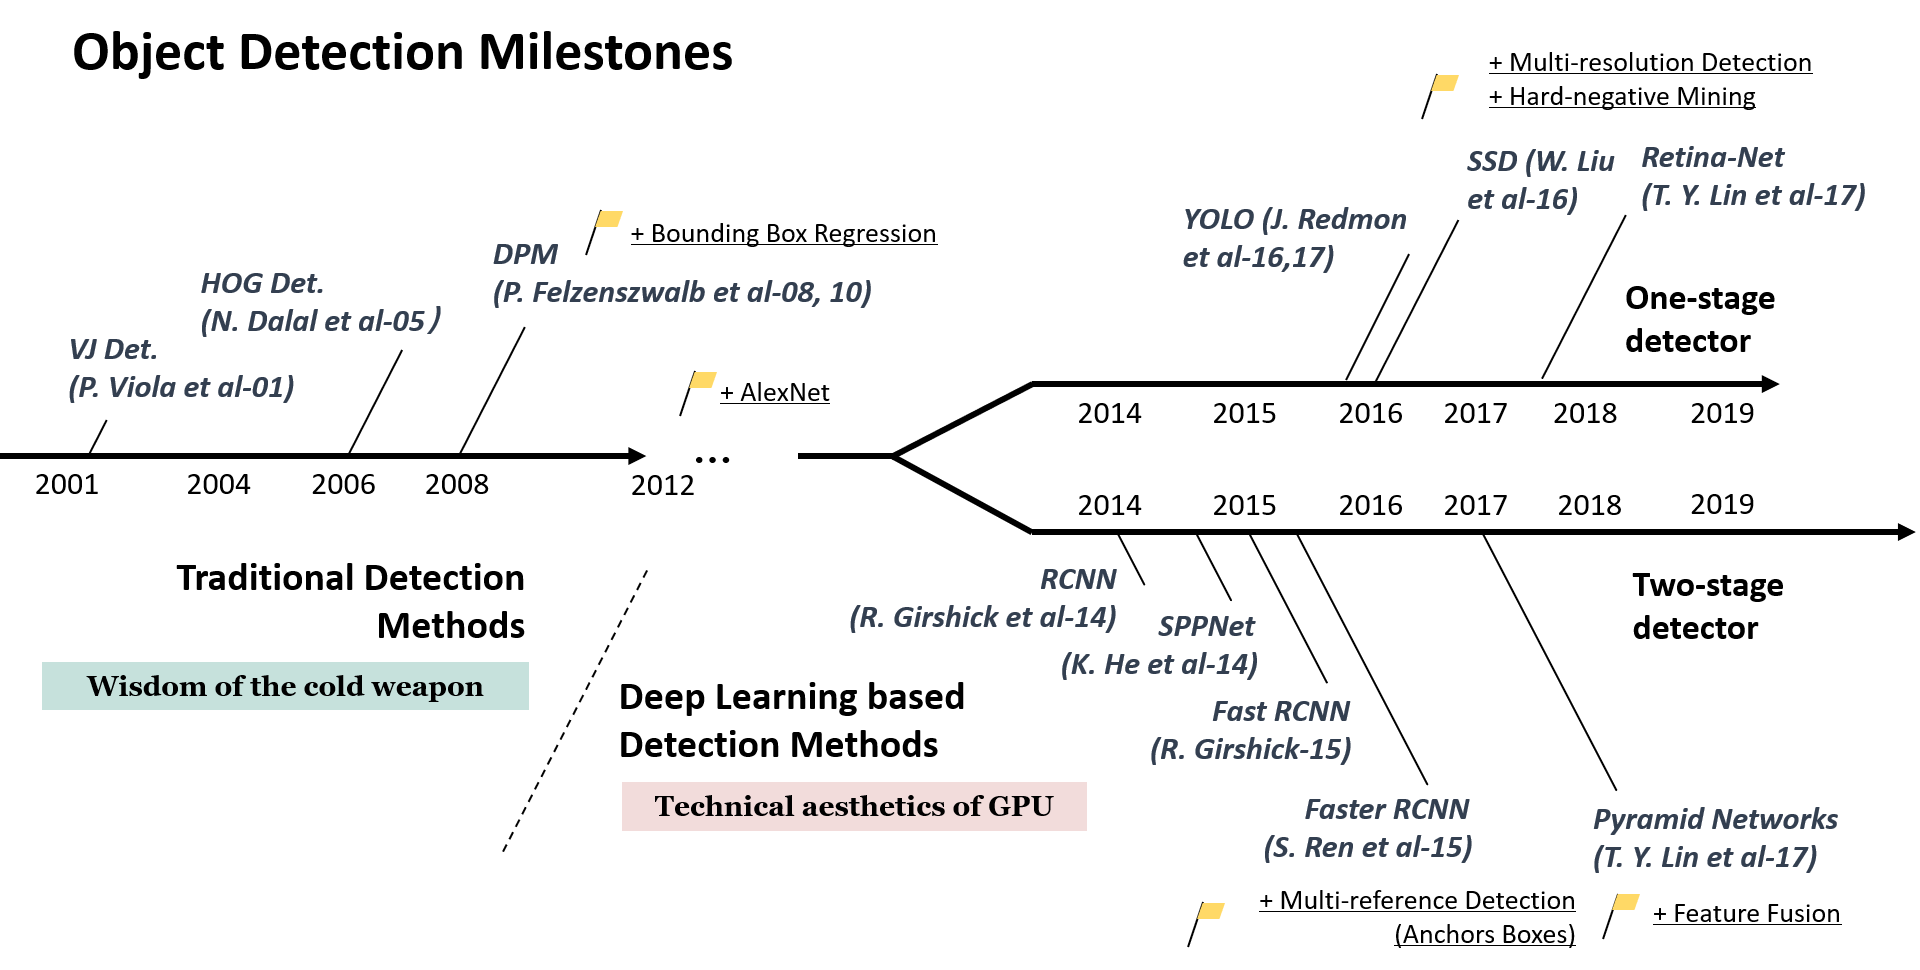
\includegraphics[width=\textwidth]{images/mile-stones.png}
    \caption{Storia della Object Detection \cite{DBLP:journals/corr/abs-1905-05055}}
    \label{fig:history_object_detection}
\end{figure}
\subsection{Evoluzione delle tecniche}
Durante questo ventennio i detector più famosi sono stati costruiti usando come mattoncini delle tecniche sviluppate ed affinate via via nel tempo. Queste tecniche sono di diverso tipo ed hanno subito evoluzioni di cui faremo una disamina nel proseguio di questa sottosezione.
\subsubsection{Prime tecniche}
Storicamente una delle prime tecniche si basava sul una teoria cognitiva chiamata \textit{Recognition by Components} \cite{biederman1987recognition}, ed è stata per molto tempo la base di alcuni lavori riguardanti il riconoscimento di immagini e la rilevazione di oggetti \cite{felzenszwalb2008discriminatively} \cite{fischler1973representation} \cite{leibe2008robust}.   

Nel passato alcuni ricercatori hanno formulato soluzioni al problema usando misure di similarità tra le componenti di un oggetto, tra la forma o i contorni, tra cui \textit{Distance Transforms} \cite{gavrila1999real}, \textit{Shape Contexts} \cite{belongie2002shape} e \textit{Edgelet} \cite{wu2005detection}.

I risultati iniziali erano molto promettenti, tuttavia quando la rilevazione è diventata più complicata queste tecniche hanno iniziato a mostrare i propri limiti, motivo per cui il passaggio al Machine Learning è stato quasi naturale. Le prime metodologie basate su questo approccio risalgono ad un periodo inquadrabile prima del $1998$, in questo caso la detection si basava su modelli statistici costruiti sopra le apparenze degli oggetti da rilevare. 
Il primo di questi modelli statistici nasce nel $1991$, chiamato \textit{Eigenfaces} \cite{turk1991eigenfaces} \cite{pentland1994view}, riesce in laboratorio a riconoscere volti in tempo reale.

Successivamente, fino al $2005$, l'evoluzione ha portato a tecniche in cui si cambiava radicalmente la rappresentazione, intesa come feature, delle immagini. Lo scopo era quindi apprendere come trasformare un immagine da insieme di pixel a insieme di coefficenti \textit{wavelet}. Grazie alla sua efficienza, tra tutte le trasformate, quella a prendere piede fu la \textit{Haar wavelet}. Dal $2005$ al $2012$ c'è stato un passaggio a rappresentazioni basate sul gradiente. 

Intorno al $1990$ iniziano a fare capolino le prime \ac{CNN} \cite{vaillant1994original} le quali però non hanno avuto grandi applicazioni per via dell'elevato costo computazionale rispetto alle risorse disponibili ai tempi. I modelli realizzati con \ac{CNN} non potevano essere quindi molto profondi, e per questo avevano forti limitazioni. Per ridurre questo elevato costo computazionale sono stati effettuati miglioramenti come \textit{space displacement network} \cite{lecun1998gradient}. Tramite questi perfezionamenti si è arrivato ad estendere ogni layer della \ac{CNN} in maniera tale da riuscire ad estrarre le feature da un immagine in un solo passaggio. Queste possono essere considerate un po' le antenate di quelle che attualmente chiamiamo \ac{FCN} \cite{long2015fully} \cite{chen2014semantic}. 
\subsubsection{Detection multiscala}
\label{subsec:multiscale_detection}
Uno degli aspetti più interessanti della ricerca si basa sulla rilevazione di oggetti con diverse misure o diverse proporzioni. Come è possibile bedere in Figura \ref{fig:multi_scale_history} la soluzione a questo problema ha attraversato varie fasi.
\begin{figure}
    \centering
    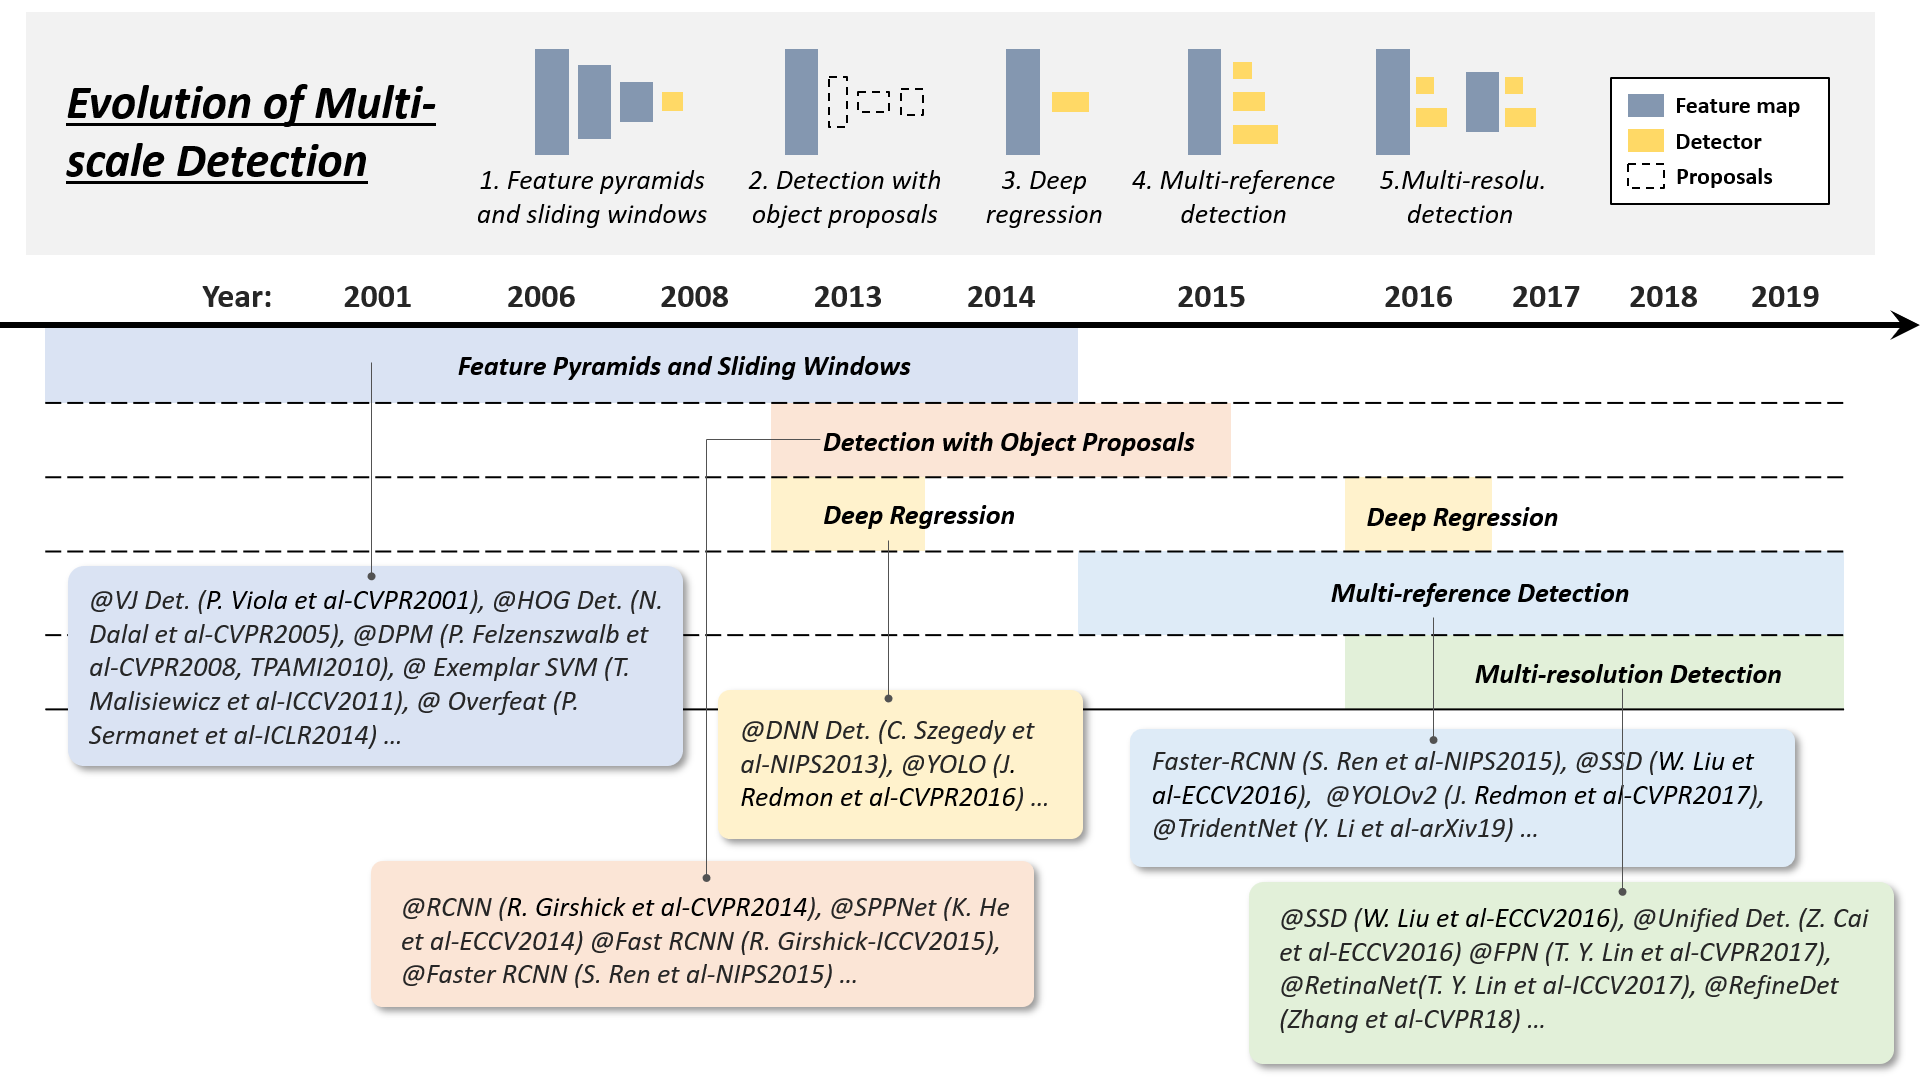
\includegraphics[width=\textwidth]{images/evol-multiscale.png}
    \caption{Evoluzione della detection multiscala \cite{DBLP:journals/corr/abs-1905-05055}}
    \label{fig:multi_scale_history}
\end{figure}
\paragraph{Feature piramidali e finestre scorrevoli}
L'idea dietro questa tecnica è abbastanza basilare, infatti dopo aver estratto le feature da un'immagine quello che viene fatto è far scorrere una finestra rettangolare di dimensione generalmente fissa per effettuare il rilevamento e la classificazione di oggetti. 

Dal $2004$ al $2014$ sono stati creati un sacco di detector basati su questa filosofia, il problema è che erano stati disegnati con l'intento specifico di rilevare oggetti con proporzioni fisse. Ricercatori come R. Girshick \textit{et al.} iniziarono a cercare soluzioni a questo problema, arrivando a formulare un modello mistura \cite{felzenszwalb2009object} composto da più modelli addestrati su oggetti con differenti proporzioni. Sono state sviluppate anche altre soluzioni, basate questa volta sull'addestrare modelli separati per ogni istanza di oggetto dell'insieme di addestramento \cite{malisiewicz2011ensemble} \cite{malisiewicz2011exemplar}. Le limitazioni di tutte queste tecniche risidono nel fatto che i dataset più moderni sono molto diversificati, quindi nel corso del tempo queste tecniche sono diventate sempre meno precise ed utilizzabili. Ciò ha portato allo sviluppo di \textit{Object Proposal}.
\paragraph{Object Proposal}
Il primo avvistamento di \textit{Object Proposal} risale al $2010$ in un task di rilevazione di oggetti \cite{alexe2010object}.
Possiamo definire una regione come un'area di un immagine contenente pixel che hanno caratteristiche comuni tra di loro. L'idea dietro questa tecnica è creare regioni non etichettate con classi che potenzialmente possono contenere qualunque tipo di oggetto, e lo scopo è riuscire a rilevare oggetti di varie misure e scale pur non dovendo necessariamente svolgere una ricerca esaustiva con finestre scorrevoli.

Per ottenere queste regioni di pixel su un immagine ci sono vari modi, discussi in parte da J. Hosang \textit{et al.} in \cite{hosang2015makes}.
\paragraph{Deep Regression}
Questa tecnica, sviluppata dal $2013$ al $2016$ si basa sull'idea di predirre direttamente le coordinate della \ac{BB} contenente l'oggetto usando come feature quelle estratte da un modello di \textit{deep learning} \cite{redmon2016you}. Il vantaggio fondamentale di questo approccio è l'efficienza e la velocità di implementazione, mentre uno svantaggio è la bassa accuratezza di localizzazione specialmente su piccoli oggetti.
\paragraph{Multi Reference Detection}
Questo approccio è il più usato per il rilevamento di oggetti con scale differenti e si basa sull'uso di un insieme di finestre rettangolari, che possono variare in dimensione e proporzioni, applicate sull'immagine, dette anche \textit{Anchor Boxes} \cite{ren2015faster, liu2016ssd, redmon2017yolo9000}. Sulla base di queste regioni rettangolari viene poi effettuata una predizione della \ac{BB}. 
\paragraph{Multi Resolution Detection}
Negli ultimi anni un altro approccio che ha preso piede si basa sul rilevare oggetti di con dimensioni differenti a layer differenti \cite{liu2016ssd, lin2017feature, zhang2018single, cai2016unified}. Basti pensare alle \ac{CNN} che nel corso della propagazione dell'immagine in input, grazie alla loro composizione, formano una serie di feature piramidali. Diventa quindi più facile rilevare oggetti grandi nei layer più profondi e viceversa diventa più facile rilevare oggetti piccoli nei layer meno profondi. 
\subsubsection{Regressione basata su Bounding Box}
Questo insieme di metodologie ha lo scopo di affinare la posizione delle \ac{BB} basandosi sulle rilevazioni effettuate tramite \textit{Object Proposal} o \textit{Anchor Boxes}, descritte in \ref{subsec:multiscale_detection}. Uno schema riassuntivo dell'evoluzione tecnica di questi approcci è in Figura \ref{fig:bbox_history}.
\begin{figure}
    \centering
    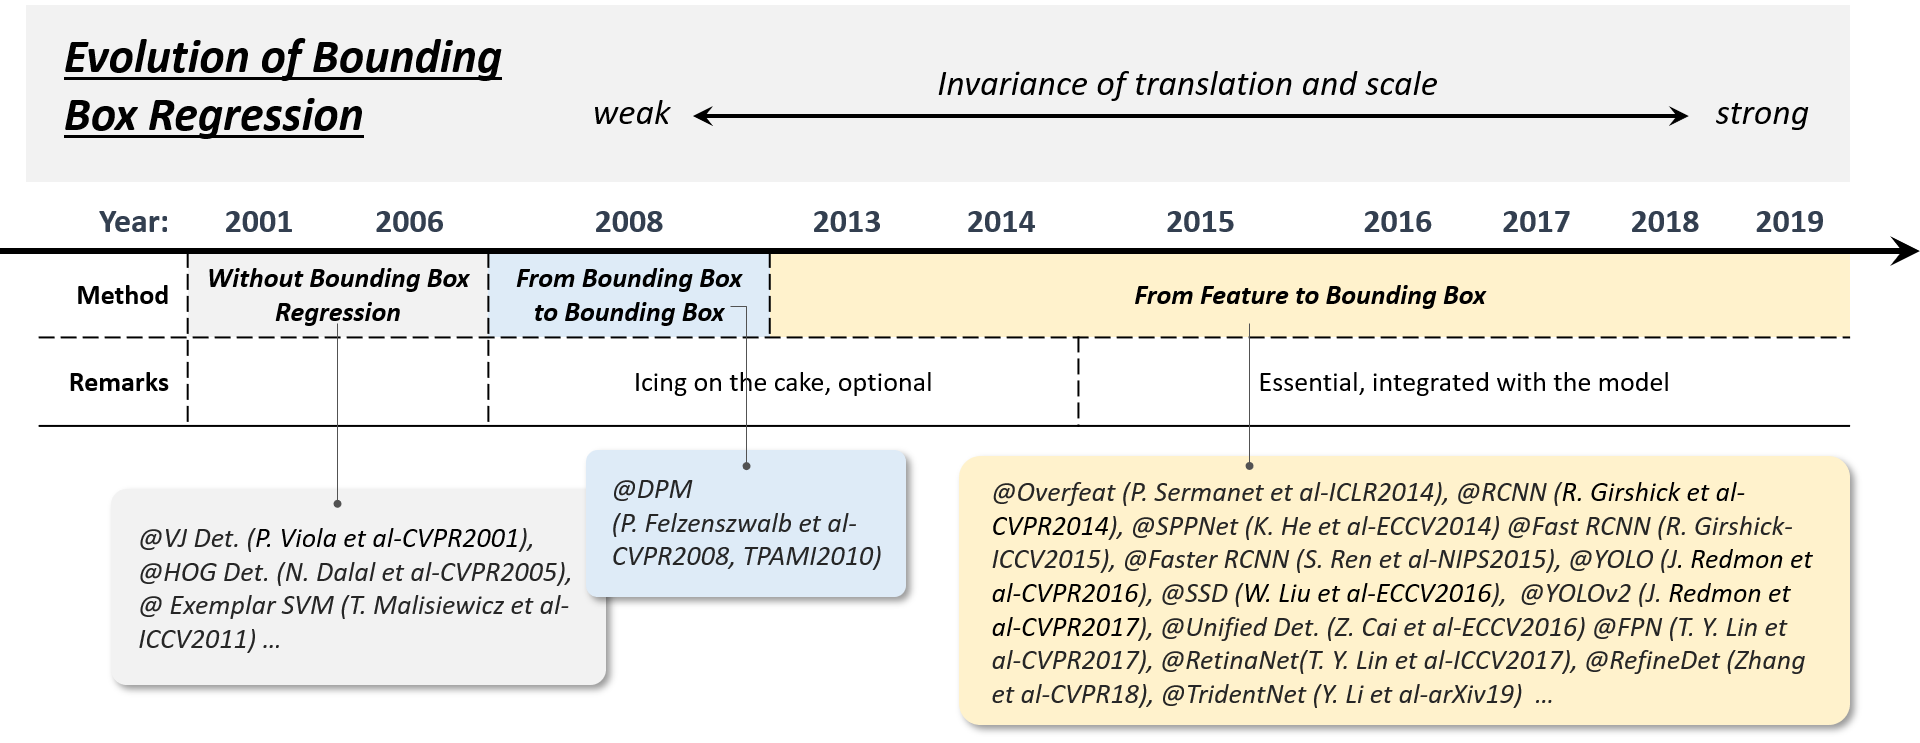
\includegraphics[width=\textwidth]{images/evol-bbreg.png}
    \caption{Evoluzione della regressione basata su \ac{BB} \cite{DBLP:journals/corr/abs-1905-05055}}
    \label{fig:bbox_history}
\end{figure}
I primi detector non raffinavano in alcun modo la posizione delle \ac{BB}, anzi molte volte usavano direttamente l'output derivato da un algoritmo basato su finestre scorrevoli. L'unico modo per ottenere rilevazioni più precise era quindi costruire modelli piramidali molto densi e assicurarsi di far scorrere la finestra lungo tutta l'immagine.
\paragraph{Da Bounding Box a Bounding Box}
I primi ad usare una forma di regressione per aumentare la precisione sulle \ac{BB} sono stati P. F. Felzenszwalb \textit{et al.} in DPM \cite{5255236} formulando la soluzione con il metodo dei minimi quadrati. Per scendere più nel dettaglio dobbiamo considerare un modello con feature piramidali.
Nel modello proposto in \cite{5255236} viene usata l'intera configurazione di $z$ per predirre la \ac{BB} riguardante quell'oggetto. In breve l'implementazione è effettuata tramite una funzione $g(z)$ che restituisce come output le coordinate $(x_1, y_1)$ e $(x_2, y_2)$ della \ac{BB}. Dopo la fase di addestramento del modello viene usato l'output di $g(z)$ per un'ulteriore fase di addestramento dove tramite il metodo dei minimi quadrati si impara a predirre $x_1, y_1, x_2 \text{ e } y_2$ partendo da $g(z)$. C'è da specificare che questo tipo di ottimizzazione è stato implementato a livello di post-processing, quindi risulta del tutto opzionale.
\paragraph{Da feature a Bounding Box}
A differenza del tipo di ottimizzazione proposto in precedenza, con l'introduzione delle \textit{Faster RCNN} \cite{ren2015faster} nel $2015$ la regressione è implementata a livello di rilevamento dell'oggetto e quindi viene addestrata insieme al modello. Inoltre, sempre confrontandolo con quanto detto prima, vengono usate anche diverse funzioni di loss da minimizzare che risultano più robuste rispetto a quella usata nei minimi quadrati. Degli esempi possono essere la \textit{smooth-L1} o la \textit{root-square}.

\subsubsection{Valutazione del contesto}
Generalmente gli oggetti che vengono rilevati dai sistemi di detection sono immersi in un contesto. Il cervello umano durante la fase cognitiva trae vantaggio dal riconoscere un contesto, motivo per cui le tecniche spiegate nel proseguio di questa sottosezione provano a emulare questa capacità degli umani. Una breve storia di come queste tecniche si sono evolute è in Figura \ref{fig:context_history}.
\begin{figure}
    \centering
    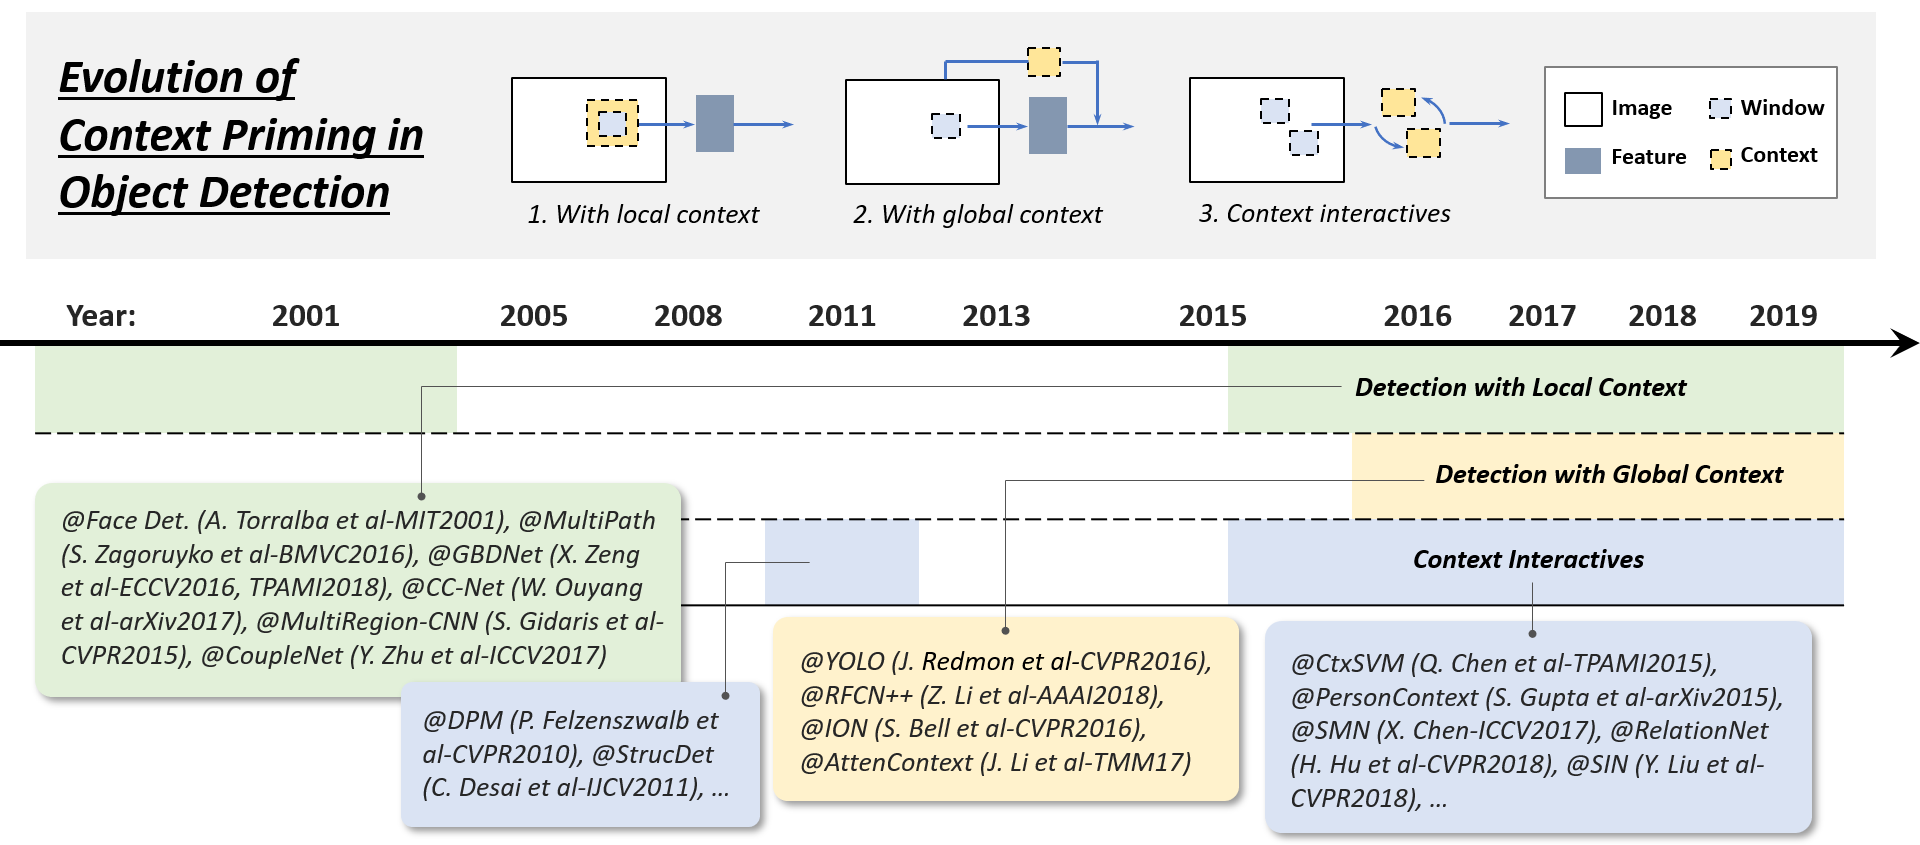
\includegraphics[width=\textwidth]{images/evol-context.png}
    \caption{Evoluzione del context priming \cite{DBLP:journals/corr/abs-1905-05055}}
    \label{fig:context_history}
\end{figure}
\paragraph{Contesto locale}
Per contesto locale si intendono tutte le informazioni visive che fanno parte dell'area prossima ai contorni di un oggetto. Sin dagli anni 2000 Sinha e Torralba in \cite{torralba2001detecting} hanno provato che includere del contesto locale migliora le prestazioni ai fini del rilevamento di volti. Dalal e Triggs in \cite{dalal2005histograms} hanno dimostrato che introdurre una piccola porzione di sfondo migliora i risultati anche nel rilevamento dei pedoni. 
\paragraph{Contesto globale}
Il contesto globale può essere considerato come una fonte di informazione aggiuntiva riguardante la scena in cui l'oggetto da rilevare è immerso. Un metodo usato all'inizio per inglobare nella detection informazioni sul contesto globale era realizzare delle statistiche che riassumevano la totalità degli elementi compresi nella scena \cite{divvala2009empirical}. In lavori più moderni catalogabili come modelli di \textit{deep learning} sono state intraprese due strade, la prima è quella di inglobare il contesto tramite campi recettivi sempre più ampi, a volte anche più dell'immagine stessa \cite{redmon2016you} o  usare l'operazione di \textit{pooling} delle \ac{CNN} \cite{li2018r}. La seconda via per ottenere informazioni dal contesto globale è pensare ad esso come un flusso di informazioni sequenziali ed usare \ac{RNN} \cite{bell2016inside, li2016attentive}. 
\paragraph{Contesto derivato dalle interazioni}
L'ultima contestualizzazione che si può dare ad un oggetto riguarda le sue interazioni con ciò che lo circonda. Per interazioni si possono intendere tutte quei vincoli o dipendenze che può avere l'obbiettivo della rilevazione. Recentemente in alcuni lavori sono state analizzate questo tipo di informazioni contestuali ai fini del miglioramento della detection. Questi miglioramenti possono essere divisi in due macrocategorie, la prima di queste è quella in cui si esplorano le relazioni tra oggetti individuali \cite{felzenszwalb2009object, desai2011discriminative, song2011contextualizing, chen2017spatial, hu2018relation}. Nella seconda categoria fanno parte i lavori nei quali vengono prese in considerazione le relazioni che ci sono tra gli oggetti e la scena che li circonda \cite{gupta2015exploring, liu2018structure}.
\subsubsection{Non Maximum Suppression}
Per \ac{NMS} si fa riferimento a tutte quelle tecniche di post processing per ridurre il fenomeno delle \ac{BB} duplicate. Questo fenomeno si concretizza quando, per la stessa rilevazione, ci sono più \ac{BB} che lo circondano con confidenze molto simili tra di loro. L'evoluzione di queste tecniche nel corso del tempo è possibile vederla in Figura \ref{fig:NMS_history}. 
\begin{figure}
    \centering
    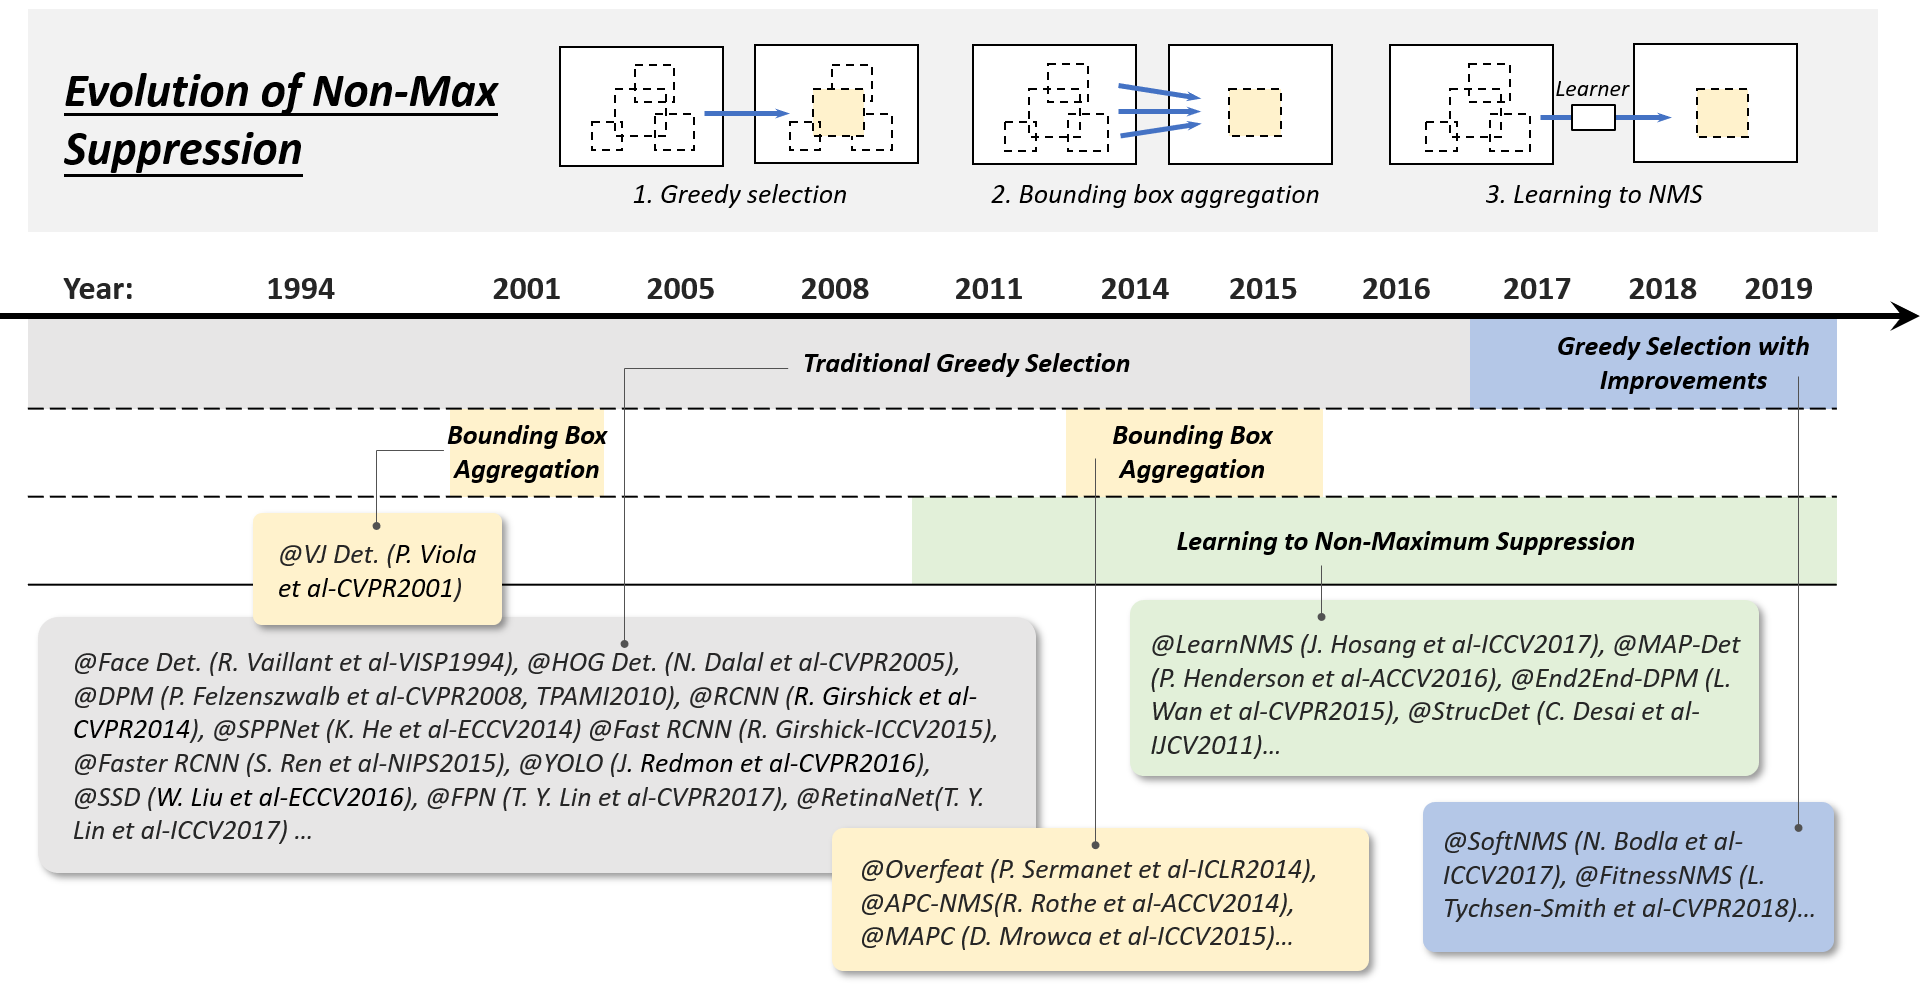
\includegraphics[width=\textwidth]{images/evol-nms.png}
    \caption{Evoluzione della Non Maximum Suppression \cite{DBLP:journals/corr/abs-1905-05055}}
    \label{fig:NMS_history}
\end{figure}


\paragraph{Greedy}
La maniera più semplice per attuare la \ac{NMS} è con un algoritmo di tipo \textit{greedy}, infatti per un insieme di \ac{BB} sovrapposte si considera solamente quella con la confidenza massima, mentre le altre vengono scartate. La sua semplicità, che da un certo punto di vista può anche essere vista come un punto di forza, può anche essere fonte di debolezze in quanto un algoritmo \textit{greedy} non sempre porta all'ottimalità. Si possono infatti verificare casi in cui la \ac{BB} con massima confidenza non ricopre tutto l'oggetto, o ancora peggio le \ac{BB} di oggetti vicini tra di loro possono essere scaratate erroneamente.


\paragraph{Aggregazione di Bounding Box}
L'aggregazione di \ac{BB} vicine tra di loro è un altro approccio per attuare la \ac{NMS} \cite{viola2001rapid, sermanet2013overfeat, rothe2014non, mrowca2015spatial}. L'aggregazione può essere fatta sia attraverso algoritmi di \textit{clustering}, sia combinando le \ac{BB} sovrapposte in un unica singola detection. 


\paragraph{Imparare ad applicare Non-maximum Suppression}
Approcci più recenti per migliorare le già sopracitate tecniche di \ac{NMS} riguardano l'apprendimento automatico \cite{wan2015end, desai2011discriminative, hosang2017learning, henderson2016end}. L'idea dietro questi metodi è trattare la \ac{NMS} alla stessa stregua di un filtro che assegna nuovi valori di confidenza a tutte le detection e quindi bisognoso di una fase di addestramento. 

\subsubsection{Hard Negative Mining}
Uno dei problemi a cui bisogna far fronte quando si tratta la \textit{Object Detection} è lo sbilanciamento tra gli oggetti che vogliamo rilevare e conseguentemente classificare e tutto quello che non ci interessa. La prima soluzione che potrebbe venire in mente per risolvere questo problema è addestrare il modello a riconoscere lo sfondo, ma questo porta a risultati distruttivi durante l'addestramento in termini di efficienza. Tecniche di \ac{HNM} servono proprio a risolvere queste problematiche. Una breve storia è possibile vederla in Figura \ref{fig:HNM_history}.
\begin{figure}
    \centering
    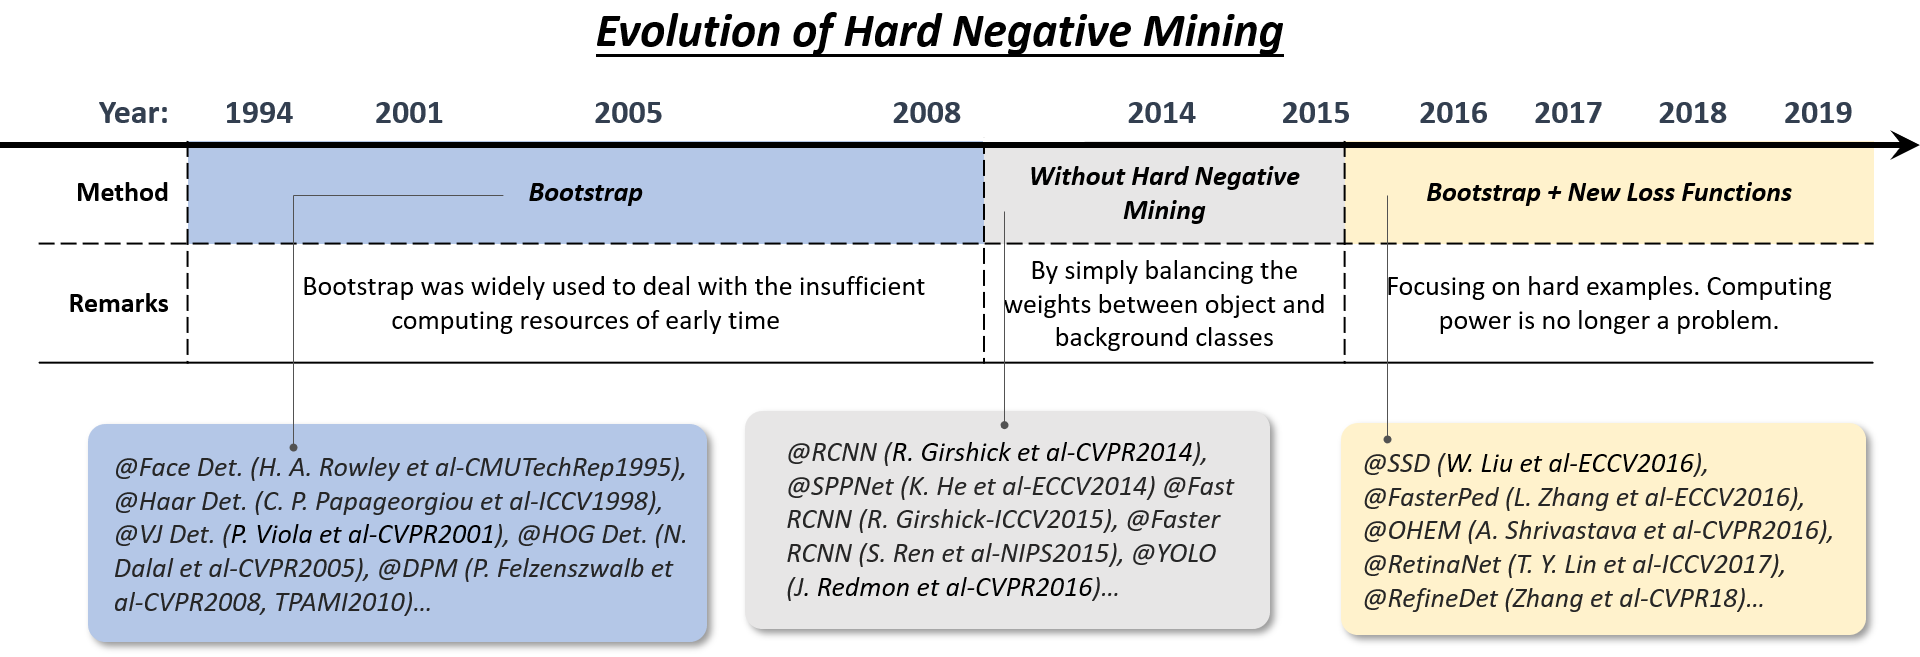
\includegraphics[width=\textwidth]{images/evol-hardnegmining.png}
    \caption{Evoluzione di Hard Negative Mining \cite{DBLP:journals/corr/abs-1905-05055}}
    \label{fig:HNM_history}
\end{figure}
\paragraph{Bootstrap}
Per Bootstrap si fa riferimento ad un gruppo di tecniche attraverso le quali si fa iniziare la fase di addestramento prendendo con dello sfondo. Successivamente quando si rilevano esempi di sfondo classificati erroneamente si aggiungono al processo di addestramento. Questo approccio risulta efficiente in quanto si evita di addestrare il modello su milioni di esempi di sfondi \cite{viola2001rapid, papageorgiou1998general, rowley1996human}.
\paragraph{HNM in detector basati su deep learning}
Recenemente modelli come Faster RCNN e \ac{YOLO} per risolvere questo problema bilanciano i pesi tra finestre con esempi negativi e positivi. Nonostante tutto però non viene risolto completamente il problema di sbilanciamento, quindi c'è stato un ritorno al \textit{bootstrap}. Un altro modo per risolvere lo sbilanciamento è l'introduzione di nuove funzioni di Loss, come ad esempio la Focal Loss in RetinaNet \cite{lin2017focal}. 




\subsection{Dataset}
L'insieme dei dati con cui addestrare e testare le performance dei modelli via via sviluppati nel corso del tempo ha subito un evoluzione. Costruire dataset sempre più grandi e con meno bias è sempre stato un obbiettivo principale che si ponevano i ricercatori, tutto ciò per realizzare dei benchmark che mettessero sempre di più a dura prova i nuovi modelli. Nel seguito di questa sezione analizzeremo in breve alcuni dei dataset più famosi nell'ambito della computer vision, con particolare attenzione per alcuni incentrati sulla rilevazione di pedoni. In Tabella \ref{table:dataset} è presente uno schema riassuntivo dei dataset analizzati nel proseguio.


\begin{table}[]
    \makebox[\textwidth]{
    \begin{tabular}{|c|c|c|c|c|c|c|}
        \hline
        \textbf{Dataset}   & \textbf{Immagini} & \textbf{Totale BB} & \textbf{Classi} & \textbf{Risoluzione} & \textbf{Fonte}       & \textbf{Altre informazioni}                                                                                  \\ \hline
        Mit ped            & 500/200           & ND                 & 1               & $64 \times 128$      & ND                   & È stato il primo                                                                                             \\ \hline
        INRIA              & 1805              & ND                 & 1               & $64 \times 128$      & ND                   & \begin{tabular}[c]{@{}c@{}}Forma rudimentale di \\ Data Augmentation\end{tabular}                            \\ \hline
        Pascal VOC (2012)  & 11540/10991       & 27450 in train     & 20              & Variabile            & Web                  & Challenge                                                                                                    \\ \hline
        Caltech            & 124K/124K         & 350K totali        & 3               & $640 \times 480$     & Vettura in movimento & Ambiente cittadino                                                                                           \\ \hline
        KITTI              & 194/195           & 160K totali        & 6               & $1382 \times 512$    & Vettura in movimento & 3D, moltissime vetture                                                                                       \\ \hline
        ILSVRC             & 458K/46K          & ND                   & 200             & Variabile            & Web                  & Challenge                                                                                                    \\ \hline
        CityPersons        & 5K                & 35K                & 4               & ND                   & Altro dataset        & \begin{tabular}[c]{@{}c@{}}\textbackslash{}ac\{BB\} con stesse proporzioni, \\ 50 città diverse\end{tabular} \\ \hline
        MS-COCO            & 123K/40K          & 896K in train      & 91              & Variabile            & Web                  & Ottima contestualizzazione                                                                                   \\ \hline
        OPEN IMAGES (2018) & 1,784M/125K       & 14M in train       & 600             & Variabile            & Web                  & \begin{tabular}[c]{@{}c@{}}Molte classi, molto ampio,\\  alta media di istanze per immagine\end{tabular}     \\ \hline
        EuroCity           & 28K/19K           & 250K in totale     & 9               & $1920 \times 1024$   & Vettura in movimento & \begin{tabular}[c]{@{}c@{}}Varietà nell'ambiente, \\ qualità delle immagini\end{tabular}                     \\ \hline
    \end{tabular}}
    \caption{Riassunto dei dataset analizzati, dove presente lo '/' indica la suddivisione tra train e test}
    \label{table:dataset}
\end{table}

\paragraph{MIT Ped.} Risale all'inizio del nuovo milleno ed è uno dei primi dataset che ha come scopo il riconoscimento di pedoni. Rispetto agli standard odierni risulta molto piccolo in quanto contiene circa 509 immagini usabili per l'addestramento e 200 usabili per la fase di test. \cite{papageorgiou2000trainable} 
\paragraph{INRIA} Risalente al 2005, nasce dall'esigenza di creare un dataset dove la detection diventasse più complicata rispetto a quello fatto dal MIT \cite{dalal2005histograms}. Contiene 1805 immagini ad una risoluzione di $64 \times 128$ pixel di esseri umani. Le immagini usate per l'insieme di training sono 2478, ovvero 1239 immagini, contenenti esempi positivi, prese dal totale più le stesse immagini ma riflesse secondo l'asse delle $y$.

\paragraph{Pascal VOC}
\ac{VOC} è collocabile in un periodo che va dal $2005$ al $2012$ \cite{everingham2010pascal, everingham2015pascal}. \ac{VOC} consiste di due parti complementari, la prima è un dataset pubblico e disponibile per esperimenti e benchmark, la seconda è una sfida annuale. Nel corso degli anni ne sono state sviluppate diverse versioni, individuabili dal pattern VOC\texttt{ANNO}. I task effettuabili su questo dataset spaziano classificazione di immagini alla object detection passando anche per il rilevamento di azioni. 
Per la sfida nel $2007$ sono state raccolte solo immagini dal social network \href{https://www.flickr.com/}{Flickr}. Le immagini sono molto variegate, ad esempio come scritto nell'articolo di presentazione del dataset \cite{everingham2010pascal} ci possono essere motociclette in diverse pose e forme, come può essere il veicolo per strada o come soggetto principale del fotogramma. 
Un altro esempio è la classe \textit{"person"}, mentre in molti dataset con questa classe ci si riferisce ad un pedone in VOC2007 con questa classe si fa riferimento ad un essere umano in diversi contesti. 
Per realizzare il dataset sono state definite delle keyword con cui effettuare query su \href{https://www.flickr.com/}{Flickr}. Queste suddette keyword sono state definite sulla base delle classi degli oggetti che si desiderava annotare. Tramite queste query sono state recuperate $500.000$ immagini, non prendendo in considerazione la data di acquisizione, il nome del fotografo, la location e via discorrendo. 
Le query venivano effettuate a gruppi di $100.000$ immagini alla volta, di cui venivano selezionate casualmente solamente alcuni fotogrammi ed inseriti nel dataset. Questa operazione è stata ripetuta fino ad ottenere la quantità desiderata di file. 
L'operazione successiva è stata quella di eliminare i duplicati o comunque immagini molto somiglianti tra di loro, una volta fatto questo sono passati ad annotarle. Di queste $500.000$ immagini agli annotatori ne sono state presentate $44.269$. Gli annotatori avevano la facoltà di scartare alcune immagini se le ritenevano non adatte ad essere annotate o avevano una confidenza bassa sull'eventuale annotazione da effettuare. Nonostante ciò è stato scoperto un'elemento che portava a del bias all'interno del dataset. L'elemento in questione riguardava il modo in cui le immagini sono state recuperate. Quando si effettua una query su \href{https://www.flickr.com/}{Flickr} il server restituisce le immagini in ordine cronologico di upload sulla piattaforma. Il dataset è stato realizzato nel Gennaio $2007$, quindi buona parte delle immagini erano ambientate in un contesto natalizio o perlopiù invernale. Con VOC2008 il problema è stato risolto aggiungendo una data casuale all'interno della query per recuperare le immagini.  

\paragraph{Caltech Pedestrian Dataset} Il \textit{Caltech Pedestrian Dataset} \cite{dollar2009pedestrian} nasce nel 2009 ed è molto più ampio di tutti gli altri dataset visti in precedenza. Le immagini sono state ricavate da circa 10 ore di video girato a 30 frame al secondo in un ambiente urbano con traffico regolare. È quindi presente un numero di frame che è nell'ordine di grandezza di $10^6$. La telecamera con cui sono state acquisite le registrazioni è stata piazzata su un'autovettura con un guidatore che attraversava le strade di Los Angeles guidando in maniera normale. La risoluzione delle immagini è di $640 \times 480$ e come conseguenza del fatto che il sistema è stato più volte smontato e rimontato ci sono piccole variazioni nella posizione della telecamera. 

Sono stati annotati $250.000$ fotogrammi, per un totale di $350.000$ \ac{BB} e $2300$ pedoni univoci. Di tutti i fotogrammi, circa il $50\%$ non hanno pedoni, mentre il $30\%$ del totale ne ha almeno due. In media un pedone è visibile per un tempo di 5 secondi. Come su dataset più recenti i pedoni sono raggruppati secondo la loro distanza dal guidatore. In particolare abbiamo che i pedoni sono vicini se la loro altezza è maggiore di $80$ pixels, sono ad una distanza media se la loro altezza è compresa tra $30$ ed $80$ pixels, mentre sono consideati lontani se la loro altezza è al più $30$ pixels. Questa discretizzazione riguardante la distanza dei pedoni è stata realizzata seguendo la distribuzione delle altezze degli stessi all'interno del dataset. Sono state inoltre prese in considerazione statistiche riguardanti l'occlusione dei pedoni e la loro posizione rispetto alla telecamera.

Il dataset è stato creato da $11$ sessioni dove in ognuna di queste venivano esplorati $5$ quartieri. Dopodiché le prime sei sessioni sono state destinate all'addestramento, mentre le rimanenti cinque sono state adibite a test set.

\paragraph{KITTI}  \cite{geiger2012we} Questo dataset è realizzato a partire da hardware usato per la guida autonoma. La particolarità è che offre informazioni tridimensionali dell'ambiente grazie a dei sensori laser dedicati che mappano il territorio circostante. Per la realizzazione sono state quindi utilizzate due telecamere a colori con una risoluzione di $1392 \times 512$ pixels, uno scanner laser ed un localizzatore GPS con un'unità di correzione RTK, il tutto orchestrato da un calcolatore su cui girava un database in real time.  Tutto questo hardware è stato montato su una station wagon che è stata guidata per dei normali scenari cittadini. 
Inoltre le annotazioni non sono \ac{BB} in due dimensioni, ma bensì dei parallelepipedi che avvolgono gli oggetti. Per la loro realizzazione sono stati presi annotatori umani che hanno posizionato \ac{BB} tridimensionali su oggetti come auto, furgoni, camion, tram, pedoni e ciclisti. Inoltre gli annotatori sono stati istruiti per marcare ogni \ac{BB} come visibile, semi occlusa, occlusa o troncata. 



\paragraph{ILSVRC}
Come per \ac{VOC} anche \ac{ILSVRC} \cite{russakovsky2015imagenet} è una challenge organizzata annualmente dal $2010$ al $2017$. Inoltre, sempre come per \ac{VOC} è presente un dataset pubblico disponibile per addestramenti e test. 
Come per alcuni dei dataset precedentemente introdotti le immagini state prese in parte da Flickr, con l'aggiunta però di altri motori di ricerca. In particolare andremo ad analizzare la costruzione della parte di dataset riguardante la \textit{object detection}, però il dataset contiene anche una parte dedicata alla classificazione di immagini ed un'altra parte dedicata alla rilevazione singola di oggetti all'interno dell'immagine. 

Le classi di oggetti presenti sono $200$ e sono stati scelte partendo dalle $1000$ classi usate per la classificazione di immagini. Una prima riduzione per arrivare a $494$ classi è stata inizialmente effettuata tramite l'eliminazione di label corrispondenti ad oggetti che occupavano gran parte del fotogramma o semplicemente non adatti alla \textit{object detection}. Un ulteriore operazione di unificazione tra classi simili ha portato il numero a $200$. 

Per il training set le immagini hanno tre provenienze differenti. Le prima sorgente di immagini è la parte di dataset dedicata alla rilevazione singola di oggetti. Per aggiungere ulteriori esempi negativi sono state effettuate prese immagini da motori di ricerca. Le immagini provenienti da queste due prime fonti sono state annotate solamente con un sottoninsieme delle classi totali. L'ultima sorgente di immagini è la piattaforma Flickr su cui sono state fatte query generiche. 
Riguardo invece la porzione di dataset dedicata alla validazione e al test la situazione è molto simile in quanto la fonte primaria ($77\%$) è la porzione di di \ac{ILSVRC}2012 adibita alla rilevazione di oggetti singoli, a cui però sono state sottratte le immagini nel quale gli oggetti occupavano più del $50\%$ dell'area totale del fotogramma. Per aggiungere ulteriori esempi, come per il training set, sono state effettuate interrogazioni generiche su Flickr. A differenza dell'insieme di immagini di addestramento, per la validazione e il test, sono state usate tutte e $200$ le classi disponibili. 
In totale per il traning set sono presenti circa $458.000$ immagini, mentre per il validation e test set sono presenti $46.000$ fotogrammi. 
\paragraph{CityPersons} Zhang \textit{et al. } \cite{zhang2017citypersons} propongono un nuovo dataset derivante da Cityscapes \cite{cordts2016cityscapes}, ma invece che focalizzarsi sulla segmentazione delle scene in contesti urbani CityPersons è incentrato sulla rilevazione di pedoni. Infatti per ogni frame di Cityscapes sono stati annotati esseri umani tramite \ac{BB}.

Le classi usate in questo dataset sono quattro, e variano a seconda della postura del pedone. Con \texttt{pedestrian} vengono indicate le persone in piedi, che corrono o camminano, mentre con \texttt{rider} si indicano quelle persone che sono alla guida di un mezzo a due ruote. Sono presenti altre due classi per indicare le persone sedute (\texttt{sitting person}) e persone con pose inusuali (\texttt{other person}).

Viene standardizzato il processo di annotazione dei \texttt{pedestrian} e \texttt{riders} in quanto le \ac{BB} hanno tutte la stessa proporzione ($0.41$), è quindi sufficiente tracciare una linea che va dalla testa ai piedi del pedone per generare una \ac{BB} delle giuste dimensioni. In questo modo si perfeziona l'allineamento della regione con l'oggetto da rilevare, e quindi si migliorano le prestazioni dell'eventuale modello. 
Per le rimanenti due classi invece non è stato standardizzato il processo, quindi vengono semplicemente disegnate \ac{BB} che contengono la persona. Un'altra operazione che è stata effettuata è stata ricercare tra le immagini tutte quelle \texttt{persone false} (manichini, statue, riflessi) per marcarli come regioni da ignorare. 

Il dataset è composto da $5000$ immagini, con un totale di circa $35000$ annotazioni e $13000$ regioni da ignorare. A differenza di KITTI e Caltech c'è una densità di persone per frame sette volte superiore ed il numero di individui distinti è prossimo a $20.000$, quindi rispettivamente $15$ e $3$ volte superiore.  La suddivisione tra test e train set è la stessa di Cityscapes. 
\paragraph{MS-COCO} \cite{lin2014microsoft}
Attualmente \ac{MSCOCO} grazie alla difficoltà di ottenere buone prestazioni è considerato uno dei più interessanti dataset per la \textit{object detection}. Rispetto a \ac{ILSVRC} ha meno classi, ma contiene molte più immagini ed annotazioni. Il punto di forza di questo dataset è la grande molteplicità di contesti in cui sono stati catturate le immagini e soprattutto la densità di oggetti che rispecchia in maniera del tutto similare quella del mondo reale. Inoltre una proprietà importante è che gli oggetti si trovano quasi sempre in contesti appropriati.

Andando più nello specifico ci si trova davanti ad un dataset che nella sua ultima versione ha, per la \textit{object detection}, circa $165.000$ immagini dedicate all'addestramento, e circa $160.000$ dedicate alla validazione ed al test. Le classi in totale sono $91$. In media ci sono $3.5$ categorie diverse e $7.7$ oggetti per immagine. In Figura \ref{fig:dataanalysis_coco} è presente uno schema riassuntivo delle statistiche di questo dataset, ed un altra cosa che si può notare è che, rispetto ad esempio a \ac{ILSVRC} e \ac{VOC}, ci sono molte meno immagini con una sola \ac{BB}, infatti in \ac{MSCOCO} solamente il $10\%$ rientra in questa categoria.
\begin{figure}
    \centering
    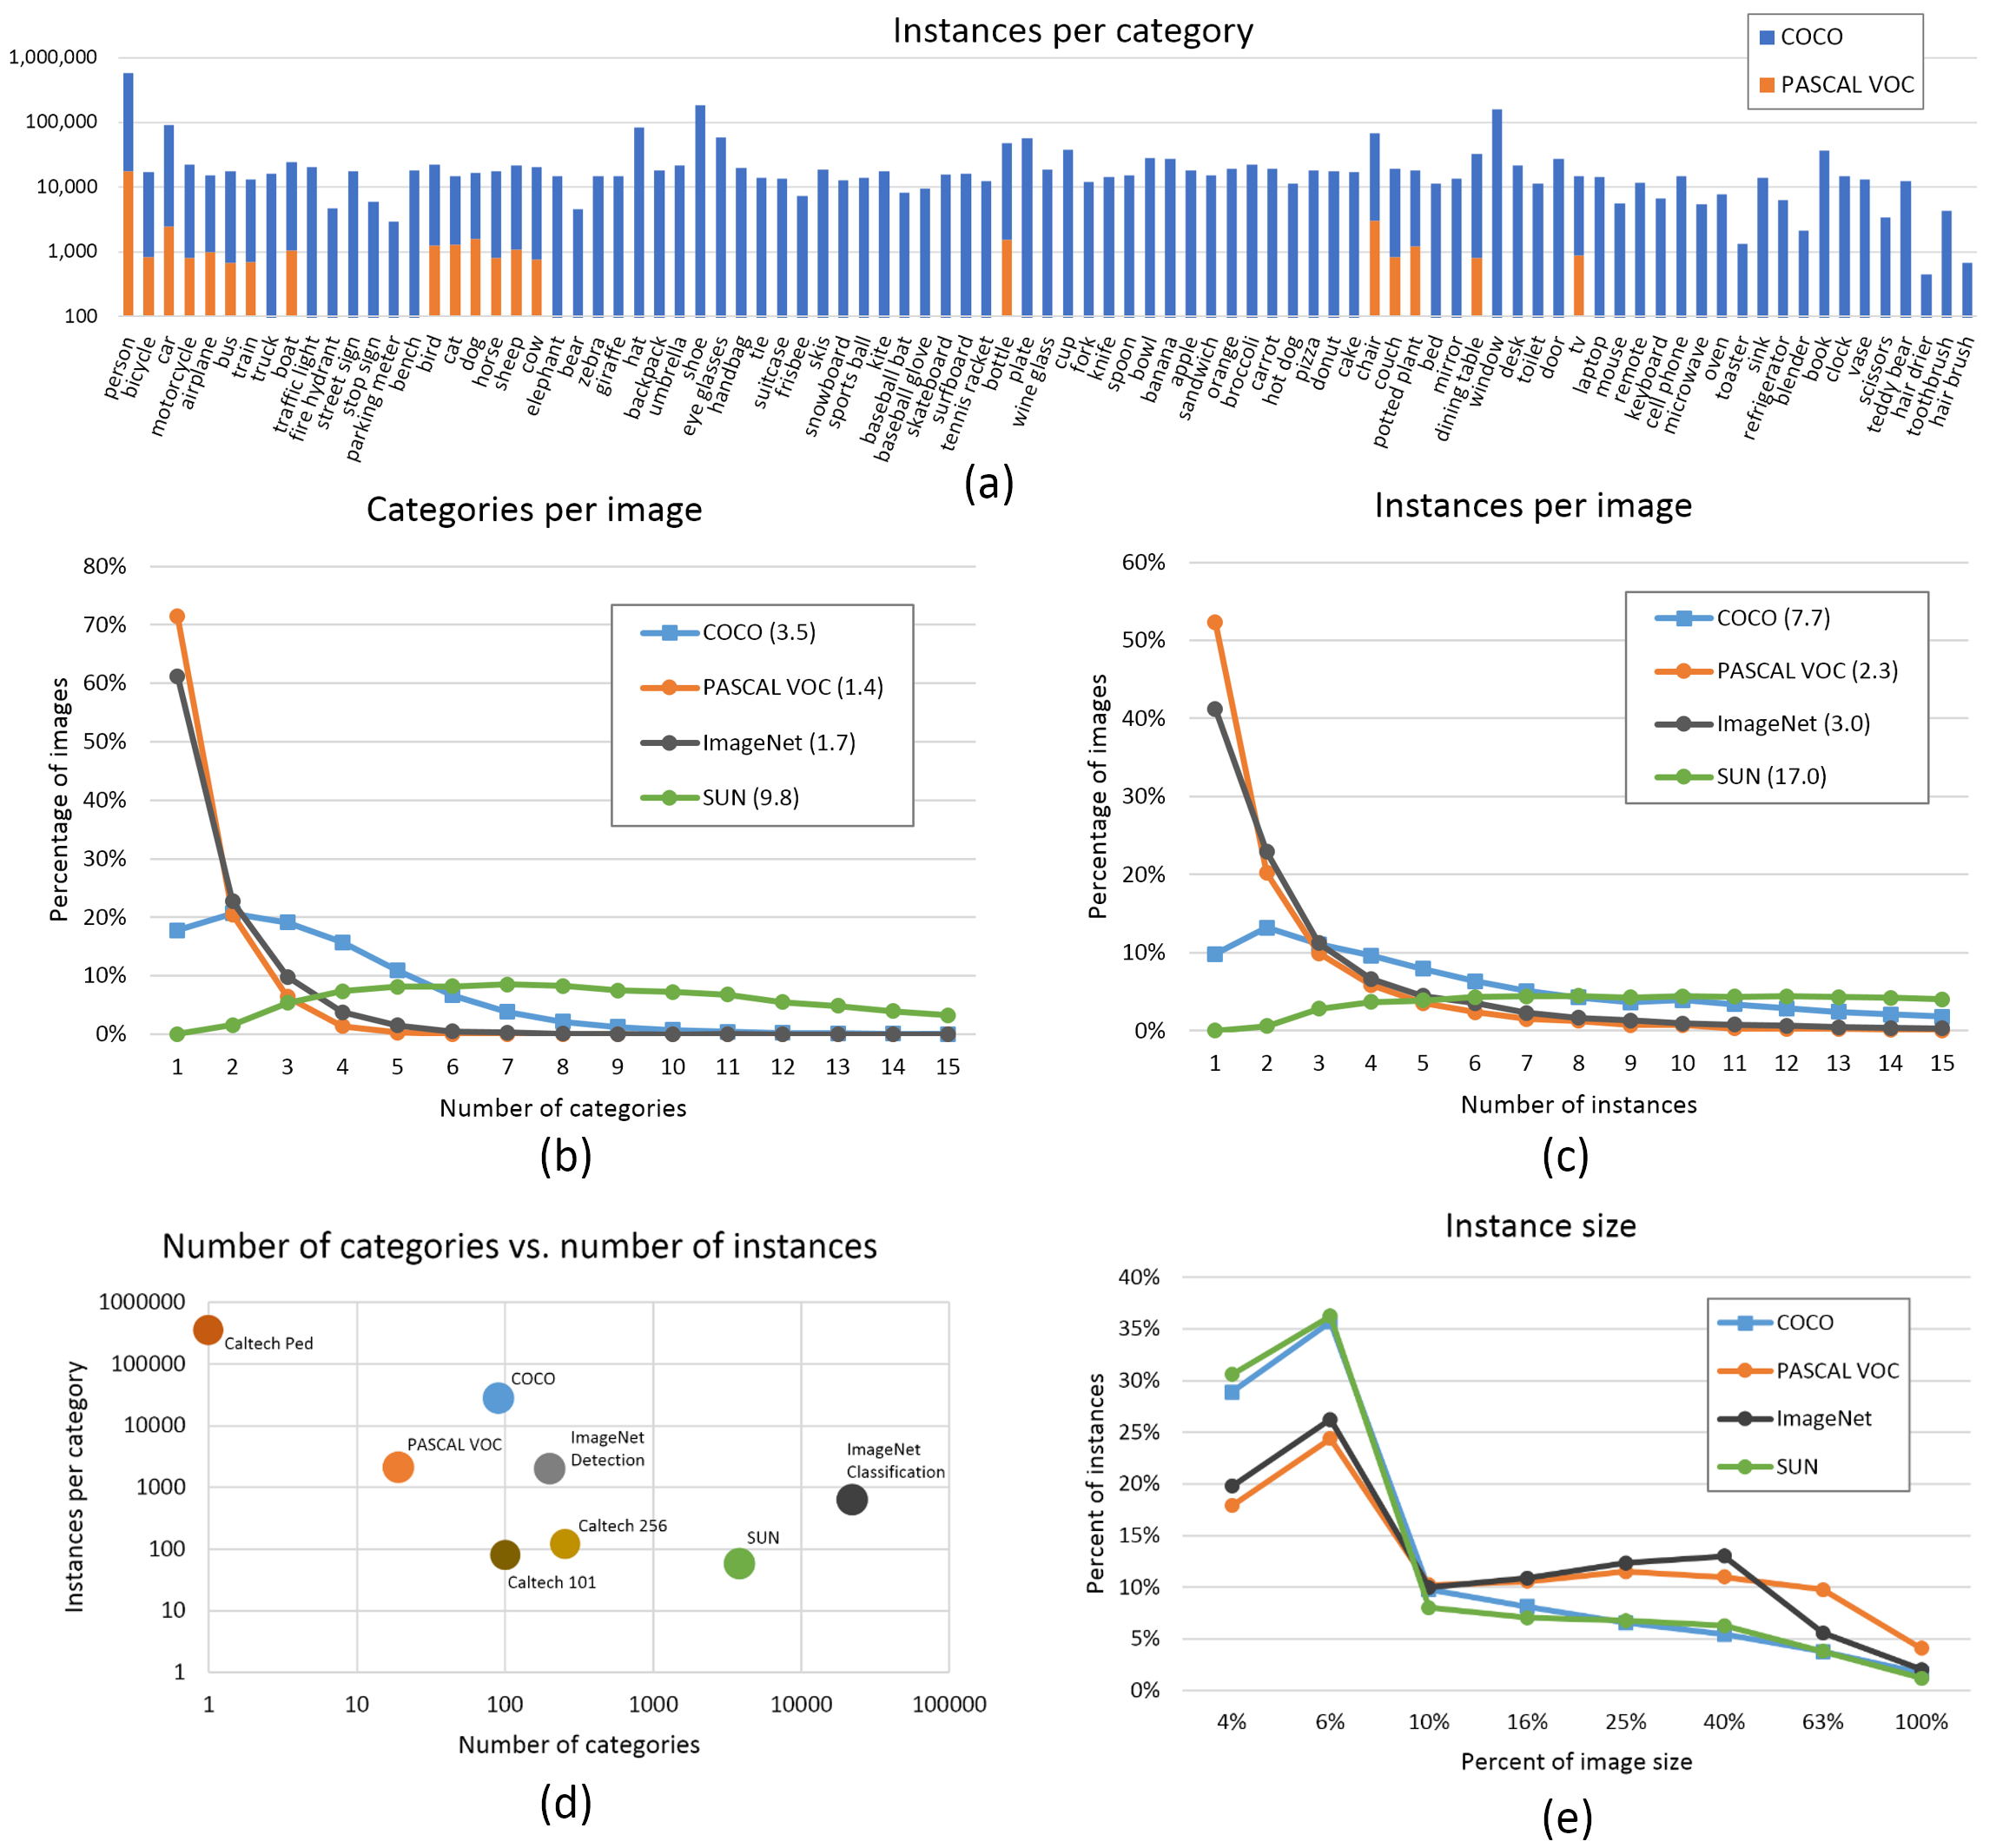
\includegraphics[width=\textwidth]{images/dataanalysis.png}
    \caption{Statistiche riassuntive di \ac{MSCOCO} \cite{lin2014microsoft}}
    \label{fig:dataanalysis_coco}
\end{figure}
\paragraph{Open Images} 
\ac{OID} \cite{krasin2017openimages}, nella versione 5, è un dataset composto da $9.2$ milioni di immagini. Ai giorni d'oggi rappresenta una delle sfide più interessanti insieme a \ac{ILSVRC} e \ac{MSCOCO}. Come per gli altri dataset anche questo si adatta a più task poiché le annotazioni sono state effettuate a livello di singola immagine, di \textit{object detection}, segmentazione e interazioni tra oggetti. 
Analizzando l'aspetto riguardante la rilevazione di oggetti ha ancora più classi rispetto a \ac{ILSVRC} in quanto per la si arriva a $600$ differenti label su $1.9$ milioni di immagini con \ac{BB} realizzate per la maggiorparte da annotatori professionali interni a Google. In aggiunta i contesti e le ambientazioni in cui sono state catturate le immagini sono molto variegati.
\paragraph{EuroCity}  EuroCity è un dataset proposto da Braun \textit{et al. } nel 2019 \cite{braun2018eurocity}. Le immagini sono state acquisite da un veicolo in movimento in $31$ diverse città europee appartenentei $12$ differenti stati. L'arco temporale attraversa le quattro stagioni, ed anche le condizioni metereologiche, fatta eccezione per forte pioggia e tempeste di neve, sono state tutte acquisite. 
La risoluzione è di $1920 \times 1024$ con un framerate di $20$ immagini al secondo. Una particolarità delle immagini acquisite da queste telecamere è lo spazio colore che arriva a $16$ bit. Quest'alta gamma dinamica si traduce in una più alta qualità dei fotogrammi in condizioni di luce non ottimale, come può essere un controsole o una notturna. 
Per ogni città in media sono state catturate $1.7$ ore di video e le immagini sono state campionate ogni $4$ secondi ($80$ frame). Questo porta ad avere una ripetizione minore di pedoni o oggetti uguali, soprattutto in condizioni trafficate.
Le classi in questo dataset si differenziano in base al veicolo su cui si trovano i pedoni. Sono stati annotati gli esseri umani a piedi, sulle moto, scooter, tricicli, sedie a rotelle e buggy. 
L'occlusione è stata gestita decidendo di annotare l'oggetto nella sua totalità dando una misura spannometrica per le dimensioni della \ac{BB}. 
Riguardo i veicoli invece sono state fatte \ac{BB} separate per il veicolo e la persona al di sopra. 
C'è anche una parte di persone scartate che sono quelle che hanno un'altezza inferiore a 20 pixels. 


\subsection{Metriche}
\section{Detector basati su metodi tradizionali}
\label{sec:traditional_method}

\paragraph{Viola Jones Detectors}
Nel 2001 P. Viola e M. Jones \cite{viola2001rapid, viola2004robust} sono riusciti a realizzare un modello, chiamato \ac{VJ} Detector, capace di riconoscere volti umani in condizioni non vincolate. L'hardware che fu usato era al passo con i tempi, si parla infatti di un processore Intel Pentium III, ed i risultati erano impressionanti. Molti altri algoritmi di rilevazione di volti infatti giravano decine, se non centinaia, di volte più lenti rispetto ad \ac{VJ} e l'accuratezza era del tutto paragonabile. 

L'approccio usato dai due ricercatori in fase di sviluppo è anche uno dei più basilari, ovvero la finestra scorrevole. Nonostante il compito fosse molto al di la della portata dell'hardware dei tempi questo detector tramite alcune tecniche è riuscito a migliorare drasticamente la sua efficienza in termini di velocità e accuratezza. 
La prima di queste tecniche è un algoritmo chiamato \textit{integral image} che serve a computare efficentemente la somma di valori in un sottoinsieme rettangolare di una griglia. In questo modo si è riuscito a velocizzare le operazioni di filtraggio e convoluzione. 
Il secondo mattoncino con cui è stato costruito \ac{VJ} riguarda la scelta delle feature delle immagini. Le feature venivano estratte grazie alla \textit{Wavelet Haar} ed invece che selezionare manualmente i filtri è stato usato Adaboost \cite{freund1999short}. 
Infine la rilevazione veniva effettuata a cascata, in questo modo si riusciva a ridurre lo spreco di risorse evitando di passare più tempo del dovuto su porzioni di immagine dove l'algoritmo aveva una ragionevole certezza fossero sfondo. 
\paragraph{Histogram of Oriented Gradients}
\ac{HOG} è un descrittore di feature per immagini presentato nel 2005 da N. Dalal e B. Triggs \cite{dalal2005histograms}. Il suo scopo era quindi l'estrazione di informazioni utili da un immagine, cercando di scartare il più possibile informazioni inutili. La motivazione per la realizzazione è stata la rilevazione di pedoni, tuttavia è facilmente adattabile alla rilevazione di altre classi. 
L'idea dietro queste feature si basa sul gradiente secondo una direzione. Possiamo spiegarlo intuitivamente come la variazione di colore che si ha andando in una determinata direzione di una regione rettangolare dell'immagine. 
L'estrazione procede dividendo l'immagine in celle non disgiunte e per ognuna di esse osservando i pixel che la compongono si calcola un istogramma monodimensionale dei gradienti secondo le varie direzioni. Prendendo tutti gli istogrammi derivanti dalle celle si ottiene una rappresentazione sottoforma di feature \ac{HOG} dell'immagine. In Figura \ref{fig:hog} è possibile vedere un'esempio di estrazione di questo tipo di feature.
\begin{figure}[]
    \centering
    \subfloat[]{
        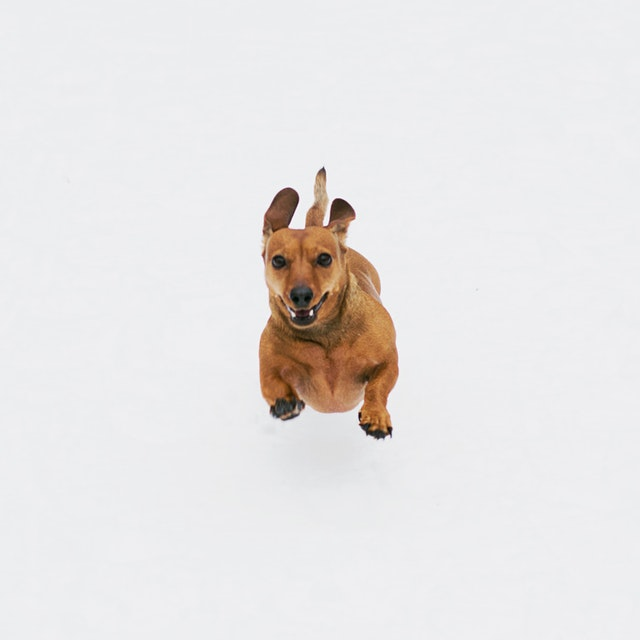
\includegraphics[width=.4\textwidth]{images/dog.jpg}
    }
    \subfloat[]{
        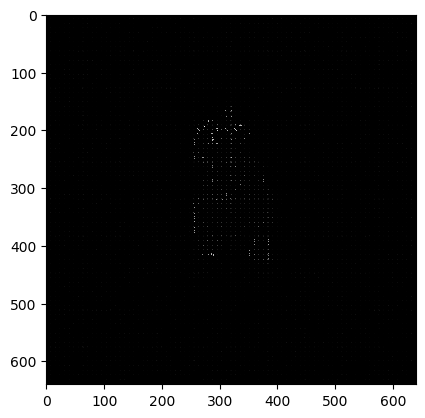
\includegraphics[width=.4\textwidth]{images/dog.png}
    }
    \caption{Esempio di estrazione feature HOG, a sinistra immagine originale, a destra dopo estrazione delle feature} 
    \label{fig:hog} 
\end{figure}

\paragraph{Deformable Part-based Model} 
La realizzazione di \ac{DPM} parte da P. Felzenszwalb nel 2005 come estensione di \ac{HOG} \cite{felzenszwalb2008discriminatively}. Questo detector è di tipo \textit{"Divide et Impera"} in quanto la fase di addestramento può semplicemente essere considerata come l'apprendere la decomposizione di un oggetto in più parti, mentre la fase di inferenza può essere vista intuitivamente come il rilevamento delle parti di un oggetto. 
Successivamente R. Girshick ha esteso questo modello, detto \textit{star-model}, ad un modello mistura \cite{felzenszwalb2010cascade, felzenszwalb2009object, girshick2011object, girshick2012rigid}. In questo modo si è riusciti ad applicare \ac{DPM} a casi reali. Per molti anni è stato considerato un punto di riferimento in quanto vincitore della sfida \ac{VOC} dal 2007 al 2009.

\ac{DPM} è formato da un filtro posizionato alla radice, più tanti altri filtri sottostanti adibiti al riconoscimento delle varie parti che formano un oggetto. Nel modello mistura di Girshick, invece che specificare manualmente cosa dovessero rilevare questi sottofiltri, venivano implementati come variabili latenti e come tali avevano bisogno di una fase di apprendimento supervisionato. 
\section{Detector basati su Deep Learning}
\label{sec:deep_learning_obj}
Come è possibile vedere da Figura \ref{fig:history_object_detection} gli anni tra il $2012$ ed il $2014$ hanno segnato un punto di svolta nella \textit{object detection} grazie a nuovi modelli basati su tecniche di apprendimento profondo. L'era attuale in cui il deep learning ha preso il sopravvento vede una diramazione nelle tecniche sviluppate per la rilevazione degli oggetti, nonostante ciò i due rami sono complementari e sviluppati in parallelo in quanto oggetto di studi recenti. La prima diramazione è quella dei detector \textit{One Stage}, questi detector ottengono prestazioni in inferenza molto elevate, a discapito però di accuratezza e e precisione nella localizzazione più scarse rispetto ai detector \textit{Two Stage}, che però sono più lenti in fase di inferenza. 
\begin{figure}[]
    \centering
    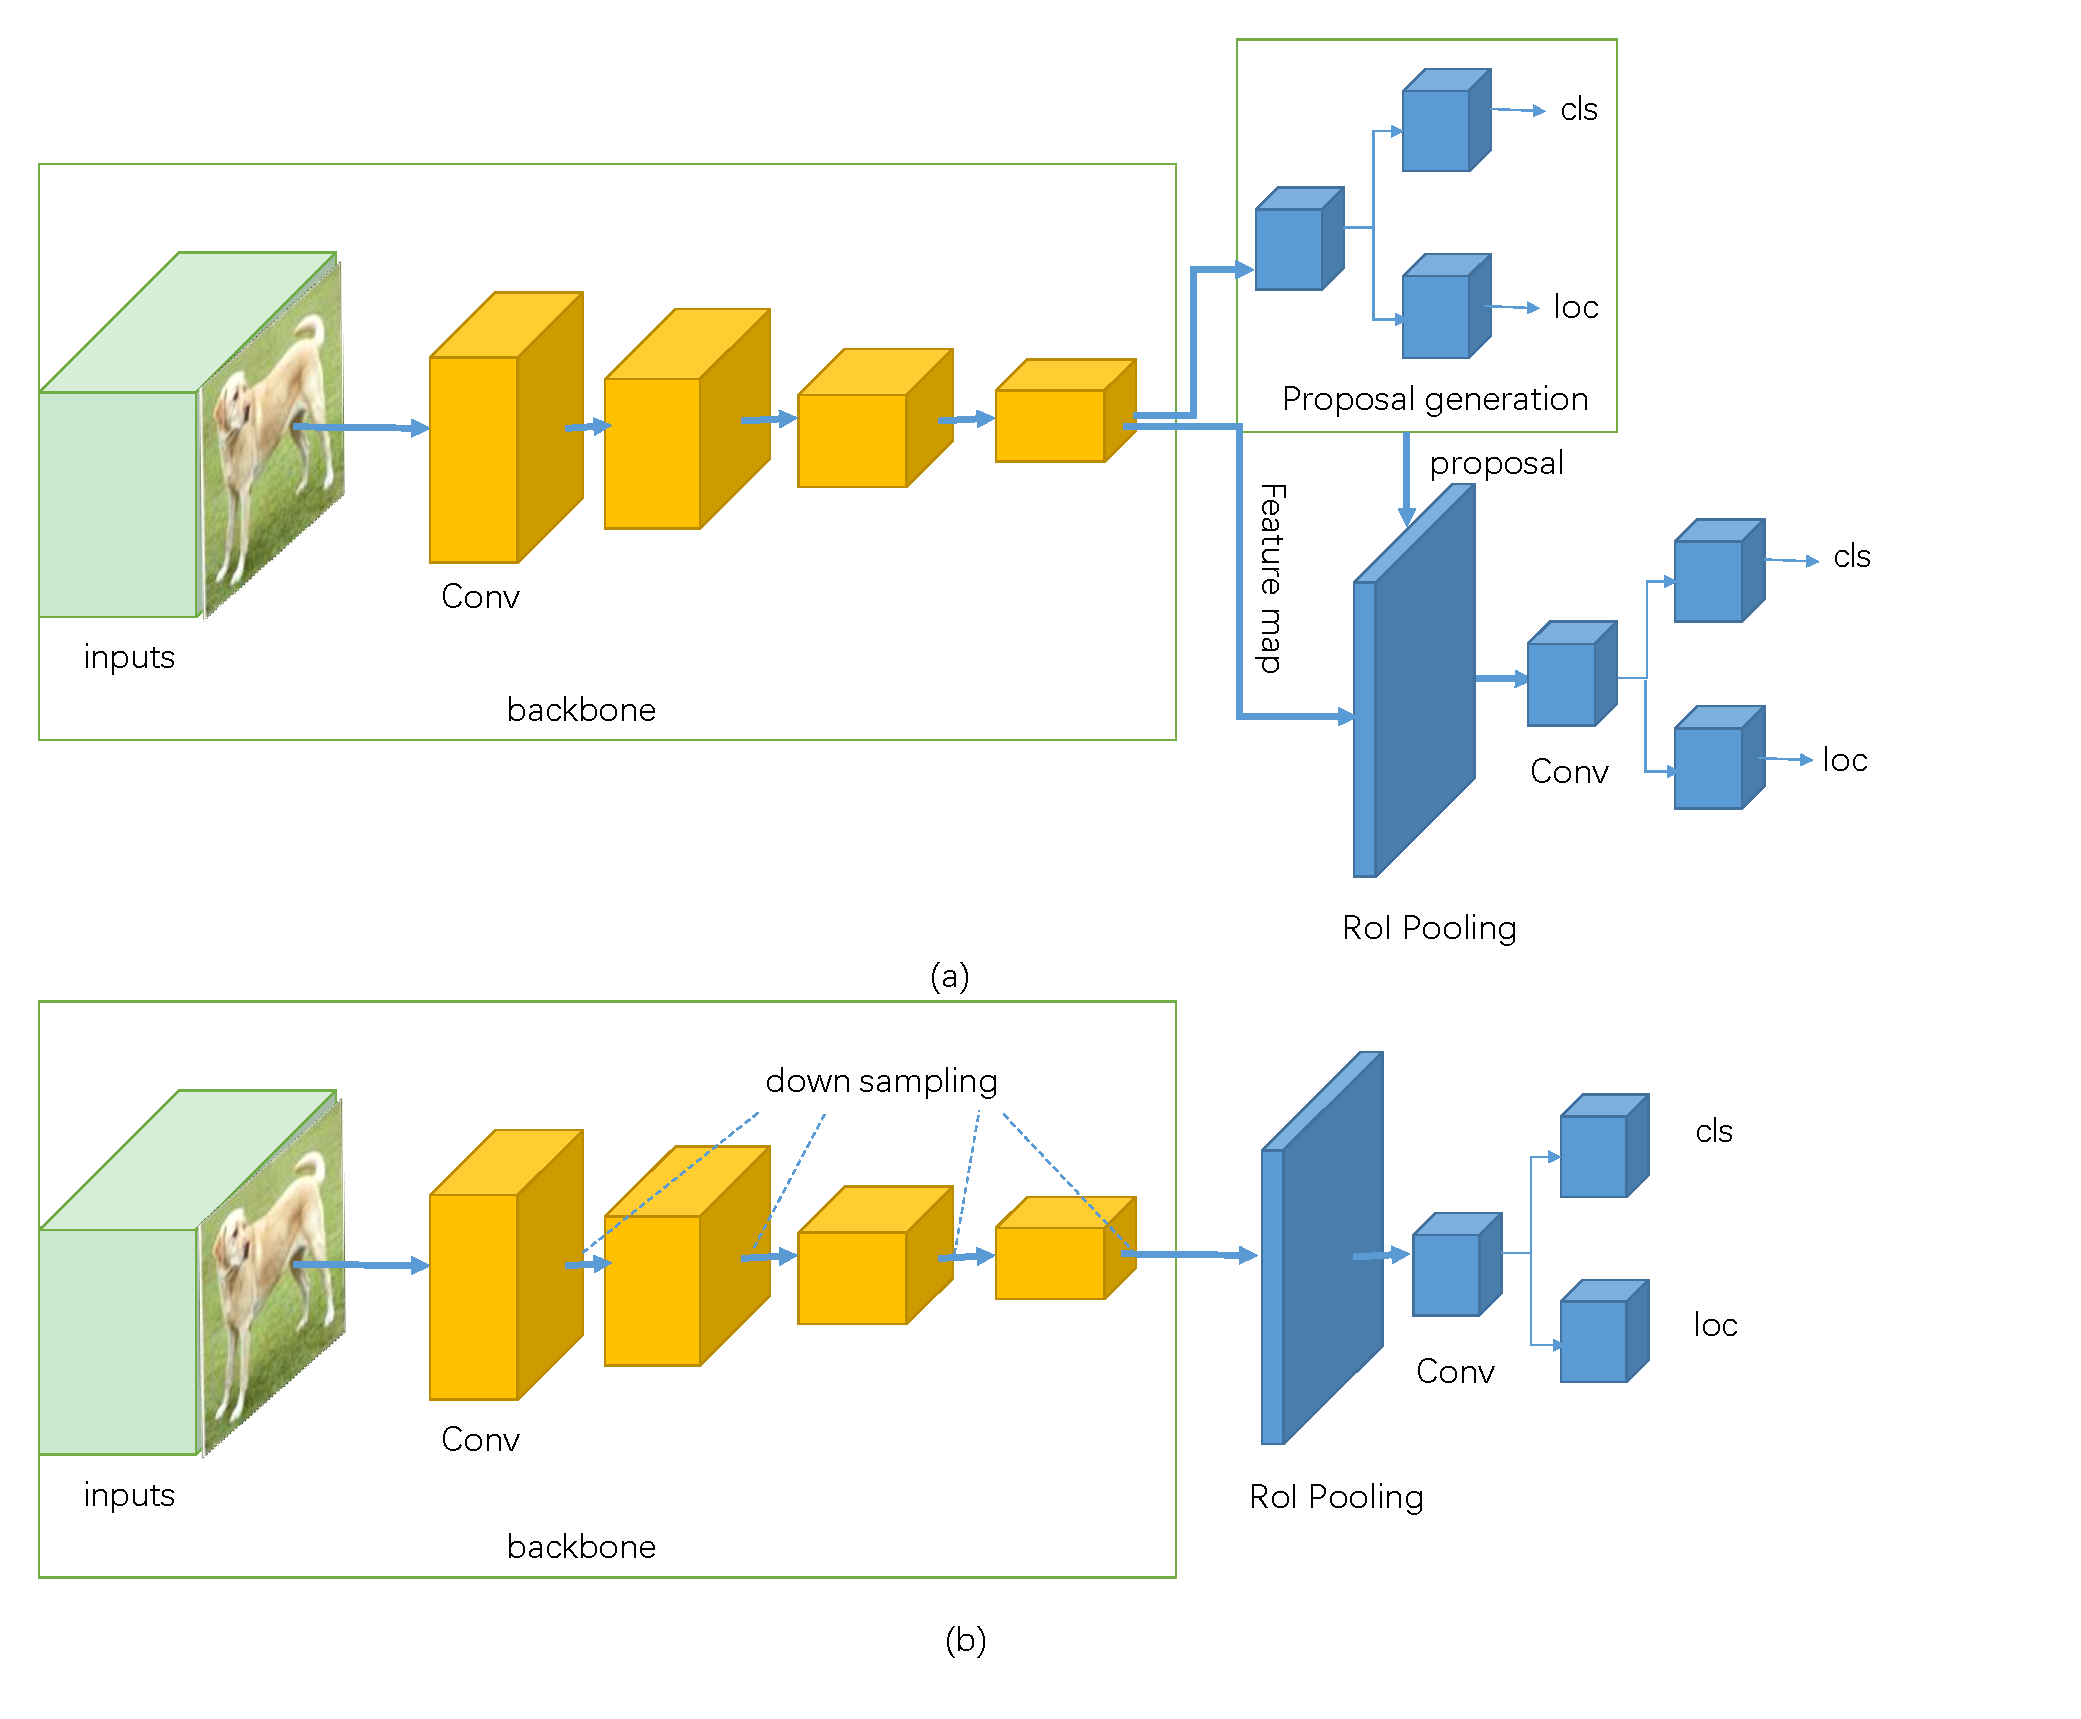
\includegraphics[width=\textwidth]{images/architectures_one_two_stage.pdf}
    \caption{In (a) la struttura di un detector a doppio stadio, in (b) la struttura di un detector a singolo stadio \cite{DBLP:journals/corr/abs-1907-09408}}
    \label{fig:detector_structure}
\end{figure}
\subsection{Estrattori di feature}
\label{sec:feature_extractor}
Nell'era dell'apprendimento profondo anche gli estrattori di feature si sono evoluti. Vengono chiamati in gergo \textit{Backbone Network} e sono reti neurali che prendono in input un'immagine e ne restituiscono le feature che poi andranno in input al modello che si occuperà della rilevazione di oggetti. 

Molte delle reti di backbone usate attualmente sono reti create per la classificazione di immagine, ma senza l'ultimo strato usato come classificatore. Come per molti compiti anche per le estrazioni delle feature possiamo effettuare delle scelte che ci portano ad avere più accuratezza, ma minore velocità di esecuzione o viceversa. 
Reti come ResNet\cite{viola2004robust}, ResNeXt \cite{he2015spatial}, AmoebaNet \cite{girshick2015fast} sono profonde e hanno un elevato grado di connessione tra i vari neuroni, risultano quindi generalmente più accurate, ma conseguentemente avere una struttura così densa porta ad avere effetti negativi sulle prestazioni. 
Molte volte però si può sacrificare un po' di accuratezza per migliorare però la velocità, un ambito ad esempio è quello dei dispotivi portatili come possono essere gli smartphone. Reti come MobileNet \cite{ren2015faster}, ShuffleNet \cite{redmon2016you}, Squeezenet \cite{liu2016ssd} o Xception \cite{lin2017feature} sono dei backbone leggeri che possono essere usati per questo scopo. 

\subsection{Two Stage Detector}
\label{subsec:two_stage_detector}
Uno schema basico dell'architettura di un rilevatore a doppio stadio è mostrata in Figura \ref{fig:detector_structure} (a). I cubi gialli sono strati convoluzionali, chiamati blocchi, presenti nella rete di backbone. Essendo nella rete di backbone da questi blocchi si otterà una mappa delle feature, che verrà passata al \ac{ROI} pooling layer per ottenere le feature definitive. 
Le proprietà estratte a quest'ultimo passaggio, nel caso dei detector a doppio stadio, passano generalmente per una \ac{RPN} che propone delle regioni in cui potenzialmente potrebbe essere contenuto un candidato alla rilevazione. L'output della \ac{RPN} a questo punto andrà come input in dei layer convoluzionali aggiuntivi (i cubi blu di Figura \ref{fig:detector_structure}) per la classificazione.
Vedremo qui di seguito alcuni modelli a doppio stadio. In particolare in Sezione \ref{sec:retinanet} vedremo in dettaglio RetinaNet, ovvero la rete neurale usata durante il lavoro di ricerca di questa tesi.  
\paragraph{R-CNN} 
Girshick nel 2014 propone il primo detector a doppio stadio chiamato R-CNN \cite{girshick2014rich}. Il modello è composto da quattro moduli. Il primo modulo genera le cosiddette region proposal, ovvero delle regioni che potenzialmente possono contenere oggetti. Il secondo modulo, partendo da queste regioni genera dei vettori di feature di dimensione fissata (4096 elementi) usando cinque strati convoluzionali e due completamente connessi. Un problema con cui si sono scontrati gli autori in questa fase è stata che l'input di una \ac{CNN} è di dimensione fissata, mentre gli oggetti possono avere dimensioni e proporzioni differenti. È stato quindi fissato l'input della \ac{CNN} come una regione di dimensione $227 \times 227$ e per far combaciare le regioni proposte del primo modulo sono state applicate trasformazioni.
La parte di classificazione è invece appannaggio del terzo modulo, ovvero  un insieme di \ac{SVM}. Le \ac{BB} vengono infine generate tramite regressione dal quarto ed ultimo modulo. Tra le \ac{CNN} i parametri sono condivisi, mentre le \ac{SVM} usate per la classificazione sono totalmente indipendenti l'una dall'altra.

La fase di addestramento di R-CNN si fa su ogni singolo componente in maniera separata. Come prima cosa viene realizzata una fase di pre-addestramento, seguita da una fase di addestramento fine. Dopodiché si vanno ad addestrare in maniera separata i classificatori \ac{SVM} e gli strati di regressione per generare le \ac{BB}.
Riguardo la classificazione un aspetto interessante di cui tenere conto è l'applicazione della \ac{IoU} o indice di Jaccard, ovvero un valore che indica la sovrapposizione tra due regioni. Varia tra 0 e 1, con 0 quando non c'è alcuna sovrapposizione ed 1 quando la sovrapposizione è totale. La \ac{IoU} si calcola prendendo in considerazione la \ac{BB} \textit{vera} e la \ac{BB} predetta in fase di inferenza. In particolare è definita come il rapporto tra l'area di intersezione delle due regioni e l'unione delle due aree. 

\paragraph{Spatial Pyramid Pooling Networks} In R-CNN uno dei problemi era nel secondo modulo quando le \ac{CNN} richiedevano un input di dimensione fissata. Con \ac{SPPNet} \cite{he2015spatial} si risolve il problema introducendo un layer di pooling piramidale che permette alle \ac{CNN} di lavorare anche con input di dimensione differente, senza necessità di applicare trasformazioni alla regione.
Con l'uso di questo nuovo strato le feature possono essere estratte solamente una volta e dall'intera immagine, il che porta \ac{SPPNet} ad essere circa 20 volte più veloce di R-CNN, senza perdere in accuratezza. 
Nonostante ciò sono presenti lo stesso alcune problematiche infatti come per R-CNN la fase di addestramento è ancora realizzata in più passaggi.
\paragraph{Fast R-CNN}
Fast R-CNN, proposta sempre da R. Girshick, \cite{girshick2015fast} è una versione migliorata di R-CNN. Uno dei grandi difetti di R-CNN era la velocità in quanto per ogni regione candidata era necessario un passaggio sulle \ac{CNN} per estrarre le feature. 
Con Fast R-CNN le feature vengono estratte in un unico momento e dall'intera immagine e successivamente passate ad  un \ac{ROI} pooling layer che restituisce in uscita vettori di dimensione fissata da passare agli strati di classificazione e regressione. 
A differenza di R-CNN e \ac{SPPNet} l'addestramento è composto da una sola fase, e questo è reso possibile da una misura di loss comune a tutta la struttura. 
Un altro miglioramento rispetto a R-CNN, e che accomuna questo detector a \ac{SPPNet}, è che vengono preservate le informazioni spaziali delle regioni candidate in quanto non c'è più necessità di avere input di dimensione fissa per le \ac{CNN}. 

Tramite queste migliorie si ottengono vantaggi notevoli rispetto a R-CNN, sia in fase di training che di inferenza. L'addestramento da 84 ore passa a circa 9.5 ore, mentre si ha un incremento di prestazioni in fase di inferenza che arriva fino a 223 volte. 
\paragraph{Faster R-CNN}
Tre mesi dopo la presentazione di Fast R-CNN venne presentata un'ulteriore versione migliorata chiamata Faster R-CNN \cite{ren2015faster}. Il collo di bottiglia di Fast R-CNN è la generazione delle regioni candidate a contenere oggetti. Con Faster R-CNN viene risolto con l'utilizzo di una \ac{RPN}, ovvero una rete convoluzionale in grado di generare efficentemente regioni di diverse dimensioni e proporzioni. Viene quindi scartata la parte iniziale di Fast R-CNN e sostituita con questa nuova \ac{RPN} che in poche parole dice a Fast R-CNN \textit{dove guarare}.

L'input di una \ac{RPN} è un'intera immagine e l'ouput sono regioni rettangolari con un indice di appartenza ad una determinata classe. 
In più in Faster R-CNN vengono utilizzate anche le Anchor Boxes 
\paragraph{FPN}
\subsection{One Stage Detector}
\label{subsec:one_stage_detector}
Lo schema architetturale di un detector a singolo stadio è visibile in Figura \ref{fig:detector_structure} (b). Inizialmente è sempre presente un backbone che servirà ad estrarre le feature dall'immagine in input, però a differenza di \ref{subsec:two_stage_detector} non è più presente la \ac{RPN}, bensì dal \ac{ROI} pooling layer si passa direttamente a dei layer convoluzionali che si occuperanno di rilevare e classificare l'oggetto di interesse. Come detto all'inizio della Sezione \ref{sec:deep_learning_obj} la struttura dei modelli a singolo stadio li porta ad avere una accuratezza ed una precisione nella localizzazione minore rispetto alla controparte a doppio stadio. Una struttura più semplice dal punto di vista degli strati però porta ad avere maggiore velocità di elaborazione. Di seguito vedremo alcuni dei più famosi modelli a singolo stadio. 
\paragraph{YOLO}
\paragraph{SSD}
\paragraph{DSSD}
\paragraph{M2DET}
\paragraph{RefineNet}

\section{RetinaNet}
\label{sec:retinanet}
\subsection{Focal Loss}